\subsection{Metrics}

To determine the performance of the feature-based approach, the matching of keypoints is framed in terms of a binary classifier.
For a keypoint correspondence between two images the classification task is to determine if those keypoint correspond to the same point in the real world or not.
The correspondence is computed based on the relative pose of consecutive images and only 2 consecutive images are analyzed.
This evaluation is done for \Glspl{bearing-angle-image} and \Glspl{flexion-image}.
The following subsections describe each component of this evaluation pipeline in more detail.
To the best of the author's knowledge no other work approaches the evaluation of feature detectors and descriptors like this.

\subsubsection{Groundtruth Poses}

The dataset \emph{Lehrpfad} provides groundthruth poses from a prior \gls{sfm} reconstruction.
Due to the global optimization of the \gls{sfm} algorithm these poses do not match with the depth values of the depth images.
The other dataset do not contain a precomputed pose.
Each pose is computed and refined with an ICP algorithm, namely OpenCV's \emph{FASTICPOdometry} that is based on the KinectFusion\cite{newcombe_ismar2011} work.
This relative pose serves as foundation of the evaluation and is assumed to be correct within small tolerance.
The accuracy assumption of the \emph{FASTICPOdometry} poses is tested by manual inspection of the backprojection of obviously related keypoints and the results showed no systematic errornous poses.

\subsubsection{Backprojection and Distance Threshold}

In two consecutive images all keypoints are extracted with the choosen algorithm and settings.
The keypoints of the first image is projected into the view of the second images using the determined relative pose and camera model.
This gives two sets of keypoints in the second image, the keypoints detected in this frame and the keypoints detected in the previous frame, seen from this frames pose.
Assuming a correct relative pose, the corresponding keypoints have a small pixel distance between each other.
\emph{Small} is a relative value and the choosen threshold in the experiments is $2px$.
This approach can only result in a proper analysis for a sparse distribution of keypoints that actually respond to image structure and small changes in pose.
When the pose difference is big it can happen that keypoints to covered geometry get projected to the same position as some other valid keypoint.
Too many points create ambiguity with respect to the backprojection tolerance that is required due to imperfect projections of real world sensors.
\begin{figure}[H]
    

\tikzset{every picture/.style={line width=0.75pt}} %set default line width to 0.75pt        

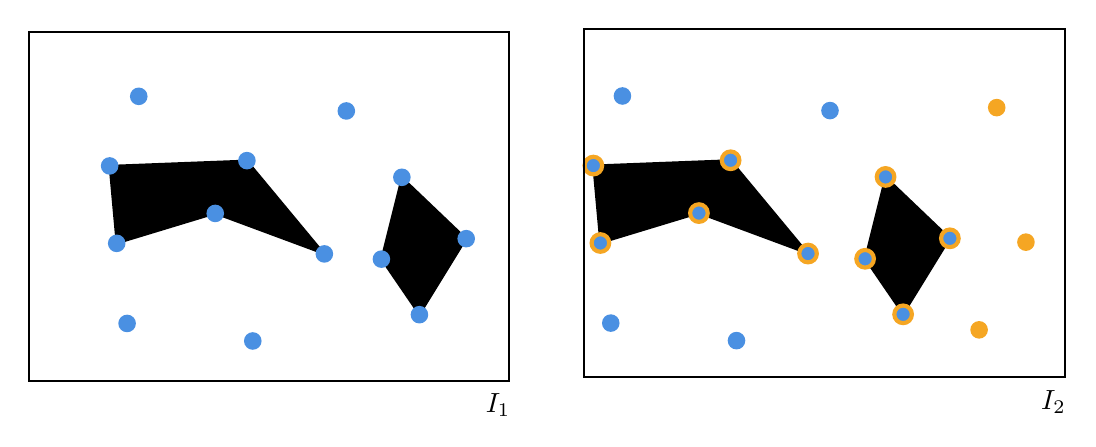
\begin{tikzpicture}[x=0.75pt,y=0.75pt,yscale=-1,xscale=1]
%uncomment if require: \path (0,229); %set diagram left start at 0, and has height of 229

%Shape: Rectangle [id:dp6786998235335104] 
\draw   (21.88,21.67) -- (253.33,21.67) -- (253.33,189.54) -- (21.88,189.54) -- cycle ;
%Shape: Polygon [id:ds4691410097865978] 
\draw  [fill={rgb, 255:red, 0; green, 0; blue, 0 }  ,fill opacity=1 ] (127.01,83.56) -- (164.31,128.49) -- (111.75,109) -- (64.27,123.41) -- (60.88,86.1) -- cycle ;
%Shape: Circle [id:dp07615520367165762] 
\draw  [draw opacity=0][fill={rgb, 255:red, 74; green, 144; blue, 226 }  ,fill opacity=1 ] (160.08,128.49) .. controls (160.08,126.15) and (161.97,124.26) .. (164.31,124.26) .. controls (166.66,124.26) and (168.55,126.15) .. (168.55,128.49) .. controls (168.55,130.84) and (166.66,132.73) .. (164.31,132.73) .. controls (161.97,132.73) and (160.08,130.84) .. (160.08,128.49) -- cycle ;
%Shape: Ellipse [id:dp6448504150595761] 
\draw  [draw opacity=0][fill={rgb, 255:red, 74; green, 144; blue, 226 }  ,fill opacity=1 ] (122.77,83.56) .. controls (122.77,81.22) and (124.67,79.32) .. (127.01,79.32) .. controls (129.35,79.32) and (131.25,81.22) .. (131.25,83.56) .. controls (131.25,85.9) and (129.35,87.8) .. (127.01,87.8) .. controls (124.67,87.8) and (122.77,85.9) .. (122.77,83.56) -- cycle ;
%Shape: Ellipse [id:dp7051810352399743] 
\draw  [draw opacity=0][fill={rgb, 255:red, 74; green, 144; blue, 226 }  ,fill opacity=1 ] (107.51,109) .. controls (107.51,106.65) and (109.41,104.76) .. (111.75,104.76) .. controls (114.09,104.76) and (115.99,106.65) .. (115.99,109) .. controls (115.99,111.34) and (114.09,113.23) .. (111.75,113.23) .. controls (109.41,113.23) and (107.51,111.34) .. (107.51,109) -- cycle ;
%Shape: Ellipse [id:dp9159085548976601] 
\draw  [draw opacity=0][fill={rgb, 255:red, 74; green, 144; blue, 226 }  ,fill opacity=1 ] (60.04,123.41) .. controls (60.04,121.07) and (61.93,119.17) .. (64.27,119.17) .. controls (66.62,119.17) and (68.51,121.07) .. (68.51,123.41) .. controls (68.51,125.75) and (66.62,127.65) .. (64.27,127.65) .. controls (61.93,127.65) and (60.04,125.75) .. (60.04,123.41) -- cycle ;
%Shape: Ellipse [id:dp49160949647303864] 
\draw  [draw opacity=0][fill={rgb, 255:red, 74; green, 144; blue, 226 }  ,fill opacity=1 ] (56.64,86.1) .. controls (56.64,83.76) and (58.54,81.87) .. (60.88,81.87) .. controls (63.22,81.87) and (65.12,83.76) .. (65.12,86.1) .. controls (65.12,88.45) and (63.22,90.34) .. (60.88,90.34) .. controls (58.54,90.34) and (56.64,88.45) .. (56.64,86.1) -- cycle ;
%Shape: Polygon [id:ds13360398877823854] 
\draw  [fill={rgb, 255:red, 0; green, 0; blue, 0 }  ,fill opacity=1 ] (201.67,91.58) -- (232.66,121.16) -- (210.12,157.78) -- (191.81,131.01) -- cycle ;
%Shape: Ellipse [id:dp8706054475141728] 
\draw  [draw opacity=0][fill={rgb, 255:red, 74; green, 144; blue, 226 }  ,fill opacity=1 ] (205.89,157.78) .. controls (205.89,155.43) and (207.78,153.54) .. (210.12,153.54) .. controls (212.47,153.54) and (214.36,155.43) .. (214.36,157.78) .. controls (214.36,160.12) and (212.47,162.01) .. (210.12,162.01) .. controls (207.78,162.01) and (205.89,160.12) .. (205.89,157.78) -- cycle ;
%Shape: Circle [id:dp6356920604931994] 
\draw  [draw opacity=0][fill={rgb, 255:red, 74; green, 144; blue, 226 }  ,fill opacity=1 ] (228.42,121.16) .. controls (228.42,118.81) and (230.32,116.92) .. (232.66,116.92) .. controls (235,116.92) and (236.9,118.81) .. (236.9,121.16) .. controls (236.9,123.5) and (235,125.39) .. (232.66,125.39) .. controls (230.32,125.39) and (228.42,123.5) .. (228.42,121.16) -- cycle ;
%Shape: Ellipse [id:dp943196171409342] 
\draw  [draw opacity=0][fill={rgb, 255:red, 74; green, 144; blue, 226 }  ,fill opacity=1 ] (197.43,91.58) .. controls (197.43,89.24) and (199.33,87.34) .. (201.67,87.34) .. controls (204.01,87.34) and (205.91,89.24) .. (205.91,91.58) .. controls (205.91,93.92) and (204.01,95.82) .. (201.67,95.82) .. controls (199.33,95.82) and (197.43,93.92) .. (197.43,91.58) -- cycle ;
%Shape: Ellipse [id:dp15135575228311182] 
\draw  [draw opacity=0][fill={rgb, 255:red, 74; green, 144; blue, 226 }  ,fill opacity=1 ] (187.58,131.01) .. controls (187.58,128.67) and (189.47,126.78) .. (191.81,126.78) .. controls (194.16,126.78) and (196.05,128.67) .. (196.05,131.01) .. controls (196.05,133.36) and (194.16,135.25) .. (191.81,135.25) .. controls (189.47,135.25) and (187.58,133.36) .. (187.58,131.01) -- cycle ;
%Shape: Circle [id:dp9787468728029534] 
\draw  [draw opacity=0][fill={rgb, 255:red, 74; green, 144; blue, 226 }  ,fill opacity=1 ] (125.6,170.45) .. controls (125.6,168.11) and (127.5,166.21) .. (129.84,166.21) .. controls (132.18,166.21) and (134.08,168.11) .. (134.08,170.45) .. controls (134.08,172.79) and (132.18,174.69) .. (129.84,174.69) .. controls (127.5,174.69) and (125.6,172.79) .. (125.6,170.45) -- cycle ;
%Shape: Circle [id:dp6723223909711141] 
\draw  [draw opacity=0][fill={rgb, 255:red, 74; green, 144; blue, 226 }  ,fill opacity=1 ] (65.04,162) .. controls (65.04,159.66) and (66.94,157.76) .. (69.28,157.76) .. controls (71.62,157.76) and (73.52,159.66) .. (73.52,162) .. controls (73.52,164.34) and (71.62,166.24) .. (69.28,166.24) .. controls (66.94,166.24) and (65.04,164.34) .. (65.04,162) -- cycle ;
%Shape: Ellipse [id:dp7974562368161737] 
\draw  [draw opacity=0][fill={rgb, 255:red, 74; green, 144; blue, 226 }  ,fill opacity=1 ] (170.66,59.62) .. controls (170.66,57.28) and (172.56,55.38) .. (174.9,55.38) .. controls (177.24,55.38) and (179.14,57.28) .. (179.14,59.62) .. controls (179.14,61.96) and (177.24,63.86) .. (174.9,63.86) .. controls (172.56,63.86) and (170.66,61.96) .. (170.66,59.62) -- cycle ;
%Shape: Ellipse [id:dp723151821080846] 
\draw  [draw opacity=0][fill={rgb, 255:red, 74; green, 144; blue, 226 }  ,fill opacity=1 ] (70.66,52.58) .. controls (70.66,50.23) and (72.56,48.34) .. (74.9,48.34) .. controls (77.24,48.34) and (79.14,50.23) .. (79.14,52.58) .. controls (79.14,54.92) and (77.24,56.81) .. (74.9,56.81) .. controls (72.56,56.81) and (70.66,54.92) .. (70.66,52.58) -- cycle ;
%Shape: Polygon [id:ds8593635117147446] 
\draw  [fill={rgb, 255:red, 0; green, 0; blue, 0 }  ,fill opacity=1 ] (360.05,83.39) -- (397.35,128.33) -- (344.79,108.83) -- (297.31,123.24) -- (293.92,85.94) -- cycle ;
%Shape: Ellipse [id:dp989610403946918] 
\draw  [color={rgb, 255:red, 245; green, 166; blue, 35 }  ,draw opacity=1 ][fill={rgb, 255:red, 74; green, 144; blue, 226 }  ,fill opacity=1 ][line width=1.5]  (393.11,128.33) .. controls (393.11,125.99) and (395.01,124.09) .. (397.35,124.09) .. controls (399.69,124.09) and (401.59,125.99) .. (401.59,128.33) .. controls (401.59,130.67) and (399.69,132.57) .. (397.35,132.57) .. controls (395.01,132.57) and (393.11,130.67) .. (393.11,128.33) -- cycle ;
%Shape: Ellipse [id:dp5019836404546896] 
\draw  [color={rgb, 255:red, 245; green, 166; blue, 35 }  ,draw opacity=1 ][fill={rgb, 255:red, 74; green, 144; blue, 226 }  ,fill opacity=1 ][line width=1.5]  (355.81,83.39) .. controls (355.81,81.05) and (357.71,79.15) .. (360.05,79.15) .. controls (362.39,79.15) and (364.29,81.05) .. (364.29,83.39) .. controls (364.29,85.74) and (362.39,87.63) .. (360.05,87.63) .. controls (357.71,87.63) and (355.81,85.74) .. (355.81,83.39) -- cycle ;
%Shape: Ellipse [id:dp7578792049912161] 
\draw  [color={rgb, 255:red, 245; green, 166; blue, 35 }  ,draw opacity=1 ][fill={rgb, 255:red, 74; green, 144; blue, 226 }  ,fill opacity=1 ][line width=1.5]  (340.55,108.83) .. controls (340.55,106.49) and (342.45,104.59) .. (344.79,104.59) .. controls (347.13,104.59) and (349.03,106.49) .. (349.03,108.83) .. controls (349.03,111.17) and (347.13,113.07) .. (344.79,113.07) .. controls (342.45,113.07) and (340.55,111.17) .. (340.55,108.83) -- cycle ;
%Shape: Ellipse [id:dp2443027365226711] 
\draw  [color={rgb, 255:red, 245; green, 166; blue, 35 }  ,draw opacity=1 ][fill={rgb, 255:red, 74; green, 144; blue, 226 }  ,fill opacity=1 ][line width=1.5]  (293.07,123.24) .. controls (293.07,120.9) and (294.97,119) .. (297.31,119) .. controls (299.65,119) and (301.55,120.9) .. (301.55,123.24) .. controls (301.55,125.58) and (299.65,127.48) .. (297.31,127.48) .. controls (294.97,127.48) and (293.07,125.58) .. (293.07,123.24) -- cycle ;
%Shape: Ellipse [id:dp9130120394048863] 
\draw  [color={rgb, 255:red, 245; green, 166; blue, 35 }  ,draw opacity=1 ][fill={rgb, 255:red, 74; green, 144; blue, 226 }  ,fill opacity=1 ][line width=1.5]  (289.68,85.94) .. controls (289.68,83.6) and (291.58,81.7) .. (293.92,81.7) .. controls (296.26,81.7) and (298.16,83.6) .. (298.16,85.94) .. controls (298.16,88.28) and (296.26,90.18) .. (293.92,90.18) .. controls (291.58,90.18) and (289.68,88.28) .. (289.68,85.94) -- cycle ;
%Shape: Polygon [id:ds05866278290858706] 
\draw  [fill={rgb, 255:red, 0; green, 0; blue, 0 }  ,fill opacity=1 ] (434.71,91.41) -- (465.7,120.99) -- (443.16,157.61) -- (424.85,130.85) -- cycle ;
%Shape: Ellipse [id:dp03726801994871687] 
\draw  [color={rgb, 255:red, 245; green, 166; blue, 35 }  ,draw opacity=1 ][fill={rgb, 255:red, 74; green, 144; blue, 226 }  ,fill opacity=1 ][line width=1.5]  (438.92,157.61) .. controls (438.92,155.27) and (440.82,153.37) .. (443.16,153.37) .. controls (445.5,153.37) and (447.4,155.27) .. (447.4,157.61) .. controls (447.4,159.95) and (445.5,161.85) .. (443.16,161.85) .. controls (440.82,161.85) and (438.92,159.95) .. (438.92,157.61) -- cycle ;
%Shape: Ellipse [id:dp8191161671737491] 
\draw  [color={rgb, 255:red, 245; green, 166; blue, 35 }  ,draw opacity=1 ][fill={rgb, 255:red, 74; green, 144; blue, 226 }  ,fill opacity=1 ][line width=1.5]  (461.46,120.99) .. controls (461.46,118.65) and (463.35,116.75) .. (465.7,116.75) .. controls (468.04,116.75) and (469.93,118.65) .. (469.93,120.99) .. controls (469.93,123.33) and (468.04,125.23) .. (465.7,125.23) .. controls (463.35,125.23) and (461.46,123.33) .. (461.46,120.99) -- cycle ;
%Shape: Ellipse [id:dp09089598583753888] 
\draw  [color={rgb, 255:red, 245; green, 166; blue, 35 }  ,draw opacity=1 ][fill={rgb, 255:red, 74; green, 144; blue, 226 }  ,fill opacity=1 ][line width=1.5]  (430.47,91.41) .. controls (430.47,89.07) and (432.37,87.17) .. (434.71,87.17) .. controls (437.05,87.17) and (438.95,89.07) .. (438.95,91.41) .. controls (438.95,93.75) and (437.05,95.65) .. (434.71,95.65) .. controls (432.37,95.65) and (430.47,93.75) .. (430.47,91.41) -- cycle ;
%Shape: Ellipse [id:dp5864704187060945] 
\draw  [color={rgb, 255:red, 245; green, 166; blue, 35 }  ,draw opacity=1 ][fill={rgb, 255:red, 74; green, 144; blue, 226 }  ,fill opacity=1 ][line width=1.5]  (420.61,130.85) .. controls (420.61,128.51) and (422.51,126.61) .. (424.85,126.61) .. controls (427.19,126.61) and (429.09,128.51) .. (429.09,130.85) .. controls (429.09,133.19) and (427.19,135.09) .. (424.85,135.09) .. controls (422.51,135.09) and (420.61,133.19) .. (420.61,130.85) -- cycle ;
%Shape: Ellipse [id:dp2039717574007679] 
\draw  [draw opacity=0][fill={rgb, 255:red, 74; green, 144; blue, 226 }  ,fill opacity=1 ] (358.64,170.28) .. controls (358.64,167.94) and (360.54,166.04) .. (362.88,166.04) .. controls (365.22,166.04) and (367.12,167.94) .. (367.12,170.28) .. controls (367.12,172.63) and (365.22,174.52) .. (362.88,174.52) .. controls (360.54,174.52) and (358.64,172.63) .. (358.64,170.28) -- cycle ;
%Shape: Ellipse [id:dp7538138790870764] 
\draw  [draw opacity=0][fill={rgb, 255:red, 74; green, 144; blue, 226 }  ,fill opacity=1 ] (298.08,161.83) .. controls (298.08,159.49) and (299.97,157.59) .. (302.32,157.59) .. controls (304.66,157.59) and (306.55,159.49) .. (306.55,161.83) .. controls (306.55,164.17) and (304.66,166.07) .. (302.32,166.07) .. controls (299.97,166.07) and (298.08,164.17) .. (298.08,161.83) -- cycle ;
%Shape: Ellipse [id:dp42526807939390865] 
\draw  [draw opacity=0][fill={rgb, 255:red, 74; green, 144; blue, 226 }  ,fill opacity=1 ] (403.7,59.45) .. controls (403.7,57.11) and (405.59,55.21) .. (407.94,55.21) .. controls (410.28,55.21) and (412.17,57.11) .. (412.17,59.45) .. controls (412.17,61.79) and (410.28,63.69) .. (407.94,63.69) .. controls (405.59,63.69) and (403.7,61.79) .. (403.7,59.45) -- cycle ;
%Shape: Ellipse [id:dp809324469000938] 
\draw  [draw opacity=0][fill={rgb, 255:red, 74; green, 144; blue, 226 }  ,fill opacity=1 ] (303.7,52.41) .. controls (303.7,50.07) and (305.59,48.17) .. (307.94,48.17) .. controls (310.28,48.17) and (312.17,50.07) .. (312.17,52.41) .. controls (312.17,54.75) and (310.28,56.65) .. (307.94,56.65) .. controls (305.59,56.65) and (303.7,54.75) .. (303.7,52.41) -- cycle ;
%Shape: Rectangle [id:dp49477644309175006] 
\draw   (289.49,20) -- (520.94,20) -- (520.94,187.86) -- (289.49,187.86) -- cycle ;
%Shape: Ellipse [id:dp012214842080934596] 
\draw  [draw opacity=0][fill={rgb, 255:red, 245; green, 166; blue, 35 }  ,fill opacity=1 ] (484.02,58.01) .. controls (484.02,55.67) and (485.92,53.78) .. (488.26,53.78) .. controls (490.6,53.78) and (492.5,55.67) .. (492.5,58.01) .. controls (492.5,60.36) and (490.6,62.25) .. (488.26,62.25) .. controls (485.92,62.25) and (484.02,60.36) .. (484.02,58.01) -- cycle ;
%Shape: Ellipse [id:dp642734465554336] 
\draw  [draw opacity=0][fill={rgb, 255:red, 245; green, 166; blue, 35 }  ,fill opacity=1 ] (498.1,122.83) .. controls (498.1,120.49) and (500,118.59) .. (502.34,118.59) .. controls (504.68,118.59) and (506.58,120.49) .. (506.58,122.83) .. controls (506.58,125.17) and (504.68,127.07) .. (502.34,127.07) .. controls (500,127.07) and (498.1,125.17) .. (498.1,122.83) -- cycle ;
%Shape: Ellipse [id:dp0666444224410937] 
\draw  [draw opacity=0][fill={rgb, 255:red, 245; green, 166; blue, 35 }  ,fill opacity=1 ] (475.54,165.08) .. controls (475.54,162.74) and (477.44,160.85) .. (479.78,160.85) .. controls (482.12,160.85) and (484.02,162.74) .. (484.02,165.08) .. controls (484.02,167.43) and (482.12,169.32) .. (479.78,169.32) .. controls (477.44,169.32) and (475.54,167.43) .. (475.54,165.08) -- cycle ;

% Text Node
\draw (240.6,194.3) node [anchor=north west][inner sep=0.75pt]   [align=left] {$\displaystyle I_{1}$};
% Text Node
\draw (508.21,192.63) node [anchor=north west][inner sep=0.75pt]   [align=left] {$\displaystyle I_{2}$};


\end{tikzpicture}


    \caption{The choosen approach of projection keypoints between frames is demonstrated in this figure. Keypoints of image $I_1$ are blue dots in both images and the oranges ones are only detected in image $I_2$. Actual correspondences result in very close points in $I_2$, indicated as blue dot with orange border, whereas unrelated points show no proximity. This assumption holds for small changes in pose and relativly sparse distribution of detected keypoints.}
\end{figure}
The analysis of the descriptor performance requires the matching step first, that establishes the correspondences of the matcher.
To classify the result of the descriptor matching, each keypoint needs to be analyzed further.
The result are four sets: \emph{true-positive}, \emph{false-positive}, \emph{true-negative} and \emph{false-negative} as introduced in Section~\ref{sec:statistic_classifier}.
The union of these sets are all detected keypoints.

Partitioning the keypoints is done with the following algorithms.
First the matches are analyzed for true and false positives and true correspondences are removed from further analysis. 
Let $proj$ be the keypoints from $I_1$, backprojected to $I_2$ with the relative pose and the appropriate camera model.
$kps$ are the keypoints from $I_2$, $matches$ are pairs of keypoints the matching algorithm considers as correspondences and $threshold$ is the maximum allowed backprojection error for keypoints to still be considered a true correspondence.
\begin{algorithm}[H]
\setstretch{1.35}
\begin{algorithmic}[0]
\Require{$\forall m \in matches \Rightarrow m.first \in proj \land m.second \in kps$}
\Require{$threshold > 0.0$}
\Ensure{$\vert true \vert + \vert false \vert = \vert matches \vert$}
    \Function{ClassifyPositives}{proj, kps, matches, threshold}
    \ForAll{$m \in matches$}
    \If{$\Call{distance}{proj[m.first], kps[m.second]} < threshold$}
        \State$true \gets true \cup m$
        \State$proj \gets proj \setminus m.first$
        \Comment{Prevent double usage}
    \Else%
        \State$false \gets false \cup m$
    \EndIf%
    \State$kps \gets kps \setminus m.second$
    \EndFor%
    \EndFunction%
\end{algorithmic}
\caption{This algorithm distinguishes between a true and a false positive match.}
\end{algorithm}
After this process some keypoints detected in $I_2$ might be left to analyze for a correspondence that was not assigned during matching, the false negatives.
\begin{algorithm}[H]
\setstretch{1.35}
\begin{algorithmic}
\Require{$threshold > 0.0$}
\Require{$kps_{pre-call}$ does not contain matched keypoints}
\Ensure{$\vert false\_negatives \vert + \vert true\_negatives \vert = \vert kps_{pre-call} \vert$}
    \Function{ClassifyNegatives}{proj, kps, threshold}
    \ForAll{$k \in kps$}
        \State$closest \gets \Call{FindClosestFrom}{proj, k}$
        \If{$\Call{distance}{closest, k} < threshold$}
            \State$false\_negatives \gets false\_negatives \cup (k, closest)$
            \State$proj \gets proj \setminus closest$
        \EndIf
    \EndFor%
    \State{$true\_negatives \gets kps \setminus false\_negatives$}
    \EndFunction%
\end{algorithmic}
\caption{After the explicit found matches are classified, the remaining keypoints need analysis to assign them as true or false positive.}
\end{algorithm}
To classify the negatives each keypoint's distance from $I_2$ to the backprojected keypoints from $I_1$ is tested to be within the defined threshold.
If this is the case, both keypoints are defined as corresponding and result in a false negative. The remaining points are true negatives.
The final partitioning of the keypoints allows to analyze more aspects of keypoints, e.g.~the descriptor distances for true and false positives.

\subsubsection{Histograms and Summary Statistics}

To visualize and understand the analyze the distribution of properties of keypoints and matches, the partitioned keypoint's are tracked in histograms.
Summary statistics reduce the statistical distributions to a few representative values.
Combining different measures, such as the measure of location, distribution and shape gives key insights.

Both histograms and its summary statistics are created for the keypoint size, keypoint response, descriptor distance between all keypoints and both descriptor distance for \emph{true-positives} and \emph{false-positives}.
The quantitive measures for each property are the \emph{minimum} and \emph{maximum} value, \emph{median} and \emph{arithmetic mean}, \emph{variance} and \emph{standard deviation} and \emph{skeweness} of the distribution.
\end{itemize}

\subsubsection{Classification Evaluation}

The analysis of the keypoint and descriptor characteristics give already some insight into the algorithm performance but are not suitable for a comparison between different algorithms and help not to find potential trade-offs.
For this task the quality of the decisions the keypoint matching algorithm is required.
The evaluation builds on the analysis of binary classifiers as introduced in Section~\ref{sec:statistic_classifier}.

The matching of descriptors is done in a simple but consistent way.
A match is defined as the closest descriptor in the other image, that also matches in the other direction.
No other criteria like a maximum matching distance is taken into account.
The matching is assessed with the computed groundtruth data.
For each obtained confusion matrix, the ratios \emph{precision}, \emph{recall} or \emph{sensitivity}, \emph{fallout} or \emph{false alarm rate}, \emph{accuracy} or the \emph{rand-index} and the \emph{youden-index} are computed at first.
For a comparison between algorithms and configurations the results are plotted in \gls{ROC}-space.
